\documentclass[12pt]{article}
\title{ECE 102 Homework 2}

\author{Lawrence Liu}
\usepackage{graphicx}
\usepackage{amsmath}
\setlength{\parskip}{\baselineskip}%
\setlength{\parindent}{0pt}%

\begin{document}
\maketitle
\section*{Problem 1}
\subsection*{(a)}
A system is linear if given that $S\{x_1(t)\}=y_1(t)$ and $S\{x_2(t)\}=y_2(t)$, we get that $S\{\alpha x_1(t)+\beta x_2(t)\}=\alpha x_1(t) +\beta x_2(t)$
\begin{align*}
S\{\alpha x_1(t)+\beta x_2(t)\}&=\int_{-\infty}^{2t}(\alpha x_1(\tau+3)+\beta x_2(\tau+3))d\tau\\
&=\alpha\int_{-\infty}^{2t}x_1(\tau+3)d\tau+\beta\int_{-\infty}^{2t}x_2(\tau+3)d\tau\\
&=\alpha y_1(t)+\beta y_2(t)
\end{align*}
Thus this system is $\boxed{\text{linear}}$.

A system is time invariant if given $S\{x(t)\}=y(t)$, $S\{x(t-\sigma)\}=y(t-\sigma)$
\begin{align*}
S\{x(t-\sigma)\}&=\int_{-\infty}^{2t}x(\tau+3-\sigma)d\tau
\end{align*}
let $\lambda=\tau-\sigma$, $d\lambda=d\tau$, and the limits of the integral become $-\infty$ to $2t-\sigma$, thus we get
$$S\{x(t-\sigma)\}=\int_{-\infty}^{2t-\sigma}x(\lambda+3)d\lambda$$
Since $y(t-\sigma)=\int_{-\infty}^{2(t-\sigma)}x(\tau+3)d\tau$ we get that the system is $\boxed{\text{time variant}}$.

This system is also $\boxed{\text{non causual}}$ since $\int_{-\infty}^{2t}x(\tau+3)d\tau$ depends on the value of $x()$ past time $t$

If $x(t)=u(t-2)-u(t-4)$ we get that 
\begin{align*}
y(t)&=\int_{-\infty}^{2t}x(\tau+3)d\tau\\
&=\int_{-\infty}^{2t}u(\tau+1)d\tau-\int_{-\infty}^{2t}u(\tau-1)d\tau\\
&=\boxed{\begin{cases}
0 & t\leq-0.5\\
2t+1 & -0.5<t\leq0.5\\
2 & t>0.5
\end{cases}}
\end{align*}
\subsection*{(b)}
A system is linear if given that $S\{x_1(t)\}=y_1(t)$ and $S\{x_2(t)\}=y_2(t)$, we get that $S\{\alpha x_1(t)+\beta x_2(t)\}=\alpha x_1(t) +\beta x_2(t)$
\begin{align*}
S\{\alpha x_1(t)+\beta x_2(t)\}&=(\alpha x_1(t)+\beta x_2(t))\sin(\pi t)\\
&=\alpha x_1(t)\sin(\pi t)+\beta x_2(t)\sin(\pi t)\\
&=\alpha y_1(t)+\beta y_2(t)
\end{align*}
Thus this system is $\boxed{\text{linear}}$.

A system is time invariant if given $S\{x(t)\}=y(t)$, $S\{x(t-\sigma)\}=y(t-\sigma)$
$$S\{x(t-\sigma)\}=x(t-\sigma)\sin(\pi t)$$
Since $y(t-\sigma)=x(t-\sigma)\sin(\pi (t-\sigma))$ we have that the system is $\boxed{\text{time variant}}$
This system is also $\boxed{\text{causual}}$ since $x(t)\sin(\pi t)$ depends only on the value of $x()$ at time $t$.

If $x(t)=u(t-2)-u(t-4)$ we get that $y(t)=\boxed{u(t-2)\sin(\pi t)-u(t-4)\sin(\pi t)}$
\subsection*{(c)}
A system is linear if given that $S\{x_1(t)\}=y_1(t)$ and $S\{x_2(t)\}=y_2(t)$, we get that $S\{\alpha x_1(t)+\beta x_2(t)\}=\alpha x_1(t) +\beta x_2(t)$
\begin{align*}
S\{\alpha x_1(t)+\beta x_2(t)\}&=\frac{d}{dt}(\alpha x_1(t)+\beta x_2(t))\\
&=\alpha\frac{dx_1(t)}{dt}+\beta\frac{dx_2(t)}{dt}\\
&=\alpha y_1(t)+\beta y_2(t)
\end{align*}
Thus this system is $\boxed{\text{linear}}$.

A system is time invariant if given $S\{x(t)\}=y(t)$, $S\{x(t-\sigma)\}=y(t-\sigma)$
\begin{align*}
S\{x(t-\sigma)\}&=\frac{d x(t-\sigma)}{dt}\\
&=\frac{d x(t-\sigma)}{d (t-\sigma)}\frac{d (t-\sigma)}{dt}\\
&=\frac{d x(t-\sigma)}{d (t-\sigma)}
\end{align*}
Since $y(t-\sigma)=\frac{d x(t-\sigma)}{d (t-\sigma)}$ therefore this system is $\boxed{\text{time invariant}}$

Furthermore, since $\frac{d x(t)}{dt}=\lim_{\Delta t\to0}\frac{x(t+\Delta t)-x(t)}{\Delta t}$ the system is $\boxed{\text{non causual}}$.

If $x(t)=u(t-2)-u(t-4)$ we get that
\begin{align*}
y(t)&=\frac{d x(t)}{dt}\\
&=\boxed{\delta(t-2)-\delta(t-4)}
\end{align*}
\subsection*{(d)}
A system is linear if given that $S\{x_1(t)\}=y_1(t)$ and $S\{x_2(t)\}=y_2(t)$, we get that $S\{\alpha x_1(t)+\beta x_2(t)\}=\alpha x_1(t) +\beta x_2(t)$
\begin{align*}
S\{\alpha x_1(t)+\beta x_2(t)\}&=\alpha x_1(2-t)+\beta x_2(2-t)+\alpha x_1(2+t)+\beta x_2(2+t)\\
&=\alpha y_1(t)+\beta y_2(t)
\end{align*}
Thus this system is $\boxed{\text{linear}}$.

A system is time invariant if given $S\{x(t)\}=y(t)$, $S\{x(t-\sigma)\}=y(t-\sigma)$
\begin{align*}
S\{x(t-\sigma)\}=x(2-t-\sigma)+x(2+t-\sigma)
\end{align*}
Since $y(t-\sigma)=x(2-(t-\sigma))+x(2+(t-\sigma))$ therefore this system is $\boxed{\text{time variant}}$

This system is also $\boxed{\text{non causual}}$ since $y(t)$ depends on values of $x()$ past time $t$, specifically $x(t+2)$.
If $x(t)=u(t-2)-u(t-4)$ we get that
\begin{align*}
y(t)&=x(2-t)+x(2+t)\\
&=u((2-t)-2)+u((t+2)-2)-u((2-t)-4)-u((2+t)-4)\\
&=u(-t)+u(t)-u(-2-t)-u(-2+t)\\
&=\boxed{0}
\end{align*}
\section*{Problem 2}
\subsection*{(a)}
\begin{align*}
y(t)&=x(t)-\int_{t-1}^{t+1}e^{|t-\tau|}x(\tau)d\tau\\
&=\int_{t-1}^{t+1}x(\tau)(\delta(\tau-t)-e^{|t-\tau|})d\tau\\
&=\boxed{\int_{-\infty}^{\infty}x(\tau)\left(\delta(\tau-t)-e^{|t-\tau|}\left(u(\tau-1)-u(\tau+1)\right)\right)d\tau}
\end{align*}
\subsection*{(b)}
A system is linear if given that $S\{x_1(t)\}=y_1(t)$ and $S\{x_2(t)\}=y_2(t)$, we get that $S\{\alpha x_1(t)+\beta x_2(t)\}=\alpha x_1(t) +\beta x_2(t)$
\begin{align*}
S\{\alpha x_1(t)+\beta x_2(t)\}&=\int_{-\infty}^{\infty}\left(\alpha x_1(\tau)+\beta x_2(\tau)\right)\left(\delta(\tau-t)-e^{|t-\tau|}\left(u(\tau-1)-u(\tau+1)\right)\right)d\tau\\
&=\alpha y_1(t)+\beta y_2(t)
\end{align*}
Thus this system is $\boxed{\text{linear}}$.

A system is time invariant if given $S\{x(t)\}=y(t)$, $S\{x(t-\sigma)\}=y(t-\sigma)$
\begin{align*}
S\{x(t-\sigma)\}&=x(t-\sigma)-\int_{t-1}^{t+1}e^{|t-\tau|}x(\tau-\sigma)d\tau
\end{align*}
$$y(t-\sigma)=x(t-\sigma)-\int_{t-1-\sigma}^{t+1-\sigma}e^{|t-\tau-\sigma|}x(\tau)d\tau$$
Let $\lambda=\tau-\sigma$, thus $d\lambda=d\sigma$ and the limits of the integral become $t-1$ and $t+1$, then we get
$$y(t-\sigma)=x(t-\sigma)-\int_{t-1}^{t+1}e^{|t-\sigma|}x(\lambda-\sigma)d\tau$$
Thus the system is $\boxed{\text{time invariant}}$

Furthermore, since $\int_{t-1}^{t+1}e^{|t-\tau|}x(\tau)d\tau$ depends on values of $x()$ past time $t$ the system is $\boxed{\text{non causual}}$.
\subsection*{(c)}
\begin{align*}
y(t)&=x(t)-\int_{t-1}^{t+1}e^{|t-\tau|}x(\tau)d\tau\\
&=\boxed{e^{-t}u(t+2)-\int_{t-1}^{t+1}e^{|t-\tau|}e^{-\tau}u(\tau+2)d\tau}
\end{align*}
\section*{Problem 3}
\subsection*{(a)}
A system is linear if given that $S\{x_1(t)\}=y_1(t)$ and $S\{x_2(t)\}=y_2(t)$, we get that $S\{\alpha x_1(t)+\beta x_2(t)\}=\alpha x_1(t) +\beta x_2(t)$. Likewise a system is time invariant if given $S\{x(t)\}=y(t)$, $S\{x(t-\sigma)\}=y(t-\sigma)$.

We can express $x_2(t)$ as $x_2(t)=x_1(t)-x_1(t-2)$. Therefore $y_2(t)=y_1(t)-y_1(t-2)$, this plot of this is drawn below
\begin{figure}[h]
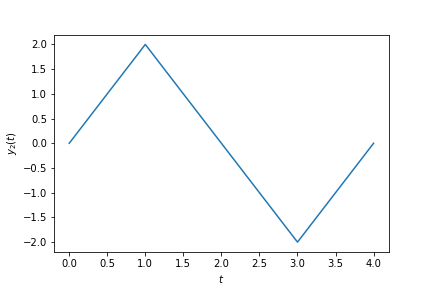
\includegraphics[scale=0.3]{fig3a}
\centering
\end{figure}
\subsection*{(b)}
We can express $x_3(t)$ as $x_3(t)=x_1(t+1)+x_1(t)$. Therefore $y_3(t)=y_1(t+1)+y_1(t)$, the plot of this is drawn below
\begin{figure}[h]
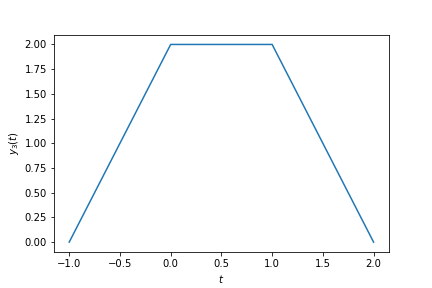
\includegraphics[scale=0.3]{fig3b}
\centering
\end{figure}
\subsection*{(c)}
\begin{align*}
h(t)&=\int_{t-2}^{t}\delta(\tau)d\tau\\
&=\boxed{u(t)-u(t-2)}
\end{align*}

Because the system is LTI to find the output of the system when the input is $x(t)=u(t+2)+u(t)-2u(t-1)+\delta(t-1)$ we just need to find the system response to a unit impulse response (which we have found) and the unit step response which is $s\{u(t)\}=\int_{t-2}^{t}=\begin{cases}
0 & t<0\\
t & 0\leq t<2\\
2 & t>2
\end{cases}$. Thus $s\{u(t+2)+u(t)-2u(t-1)\}$ looks like
\begin{figure}[h!]
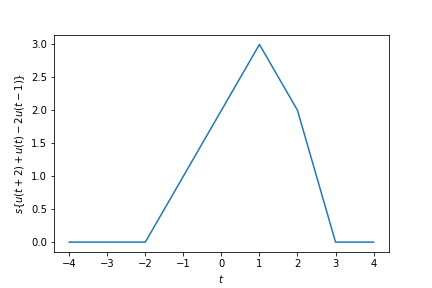
\includegraphics[scale=0.3]{fig3c}
\centering
\end{figure}
\pagebreak

And thus the system output where $x(t)=u(t+2)+u(t)-2u(t-1)+\delta(t-1)$ is
\begin{figure}[h!]
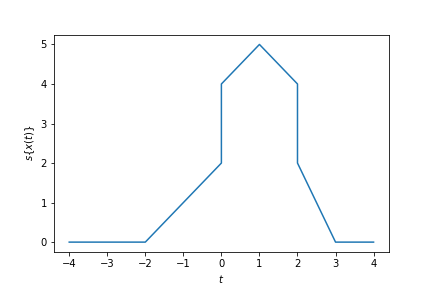
\includegraphics[scale=0.3]{fig3c2}
\centering
\end{figure}
\section*{Problem 4}
\subsection*{(a)}
\begin{align*}
h(t,\tau)=\int_{-\infty}^{\infty}e^{-t}(t-\sigma)^2u(t+\sigma)\delta(\sigma-\tau-2)d\sigma
\end{align*}
\end{document}